%%Introduction

\lettrine{T}{he} goal of this chapter is to expound on the ontology of the language, which concerns its semantics and syntactical inventory. I will achieve this by discussing the literature on various attempts and classifications proposed within the topics, and then dividing all linguistic meaning into its irreducible, unambiguous and unique atomic components, as to respect constraint 2 (unambiguity). It will use some principles of natural bifurcation of meaning (chapter 5.1.2), and built off of the universal substratum of phenomenology and qualia (chapter 5.2 and 5.3). It will also be linguistically grounded in the culturally universal basic elements of human life (chapter 5.4).


\section{Parsimony in semantics}

\subsection{\it Oligosynthesis}


Besides constraint 1 (cultural neutrality), which will be discussed in chapter 5.4, Atlan’s lexicon has to follow constraint 2 (unambiguity) and 3 (parsimony), which will be discussed in this section. Ideally, the language should contain as little basic words as possible, as to reduce the time required to learn the language. Therefore, it should be sparse with its words, only adding new words when these carry a meaning that is not already covered by another word. Complex concepts should not get their own separate words, for this would add an inestimably large number of extra words, but rather be composed of more simple and universal words that constitute its meaning. Atlan shall achieve this by using a semantic system that is oligosynthetic, meaning that it has a very limited number of semantic atoms\footnotemark (\textit{oligo}  = few), from which more complex meaning is built by combining different atoms (\textit{synthesis}  = combining). Each semantic atom (or ‘root’) shall be covered by a unique one-syllable word. Atlan syllables can take four shapes (C = some consonant, V = some vowel): V, CV, VC, CVC. This is abbreviated to (C)V(C). There are 9 consonants and 5 vowels in its phonetic inventory, yielding a total of 5 + 5x9 + 5x9 + 5x9x9 = 500 possible combinations, however all syllables ending in \textit{-ij} cannot be sufficiently distinguished by ear from those ending in \textit{-i}, so all (-) \textit{ij} will not be included. This leaves a total number of 490, and thus the challenge posed in this chapter is that of reducing all meaning to 490 atoms or a combination of these.  

\footnotetext{Throughout the book we refer to Atlans syllable words as 'semantic atoms / primes', but this definition is roughly equal to the linguistic term 'morpheme', which means as much as 'the smallest unit of meaning'. Since the atoms play a crucial role in Atlan's oligosynthetic structure, and this is not covered by the term 'morpheme' alone (which also doesn't neccesarily have to be a single syllable), we opt for this specified terminology.}

The term \textit{oligosynthetic} was first coined by the linguist Benjamin Lee Whorf and is defined as having at most a few hundred-word roots. However, this seems to be extremely rare among natural languages. A possible example might be the Kalam language of the Highlands of New Guinea (Pawley A. , 1993). Two other languages previously regarded as oligosynthetic by Whorf are the Aztec language Nahuatl and the Native American language Blackfoot, but these are now commonly classified as polysynthetic (using many roots to synthesise more complicated meaning). Oligosynthesis is more popular among constructed languages, such as Sona, Ro, aUI, Ygyde and Kali-sise (FrathWiki, Oligosynthetic language, n.d.). These all have different numbers of semantic primes and methods of synthesising them, but they commonly have the following problems (Watson, n.d.): 

\begin{itemize}
\item [I.] Complicated combinatory systems  

\item[II.] Unclear word-parsing  

\item[III.]Vagueness of composite meaning 
\end{itemize}

Atlan will overcome problem I by using an extremely basic manner of combinatory synthesis: the most semantically essential prime comes first and is followed by primes that hierarchically specify the meaning of the word. Grammatical functions always come in front of the semantic root as prefixes (except for the plural1), and semantic specifications are appended as suffixes.  

\quad
\noindent Atlan's word-composition:  

\begin{center}
{grammatical.function –  main.semantic.root – semantic.specification – plural} 
\end{center}
\quad
 

This will also solve problem II, because syllables can be recognised to be semantic when they are CVC, and grammatical otherwise. This way, grammatical syllables are easily distinguished from semantic ones. It is therefore always audibly clear where a word begins and ends. In written text this is aided by the fact that in Atlan’s own writing system, CV and VC syllables always consist of a small circle attached to a line, while CVC syllables are always two lines connected to each other.  

The 5 V syllables will be restricted to mood-markers and general sentence structuring, because of the onomatopoeic quality of these basic vocal sounds. These, however, can also be used grammatically to modify the meaning of nouns, verbs and pronouns, for example to turn ´here´ into ´where?´.  
\begin{itemize}
\item    Exclamative (prosody), imperative, vocative = o  \Atlano

\item    Interrogative (question, prosody) = e  \Atlane

\item    Stress marker (prosody) = a + stress \Atlana

\item    Relative clause = i (+ pronoun) \Atlani

\item    Subjunctive (wish) = u \Atlanu
\end{itemize}

 

The 89 CV, VC syllables will be mostly restricted to morphological and abstract functions, indicating grammatical, syntactical or logical functions and relationships between words. Logical functions will be derived from the logical operators of predicate logic and possible worlds semantics (Priest, 2011), and grammatical functions are derived from the Universal Networking Language (UNL) (Portal, sd), and syntax-semantically reduced where possible (see chapter 6.2). UNL was initiated by the United Nations University in 1996 and continued by the international non-profit organisation UNDL from 2001 onwards. Its goal is to function as a formalised pivot language between natural language and interlingual machine translation, therefore having formalised all grammatical functions, together with a large-scale ontology of all concepts contained within all its source languages (Universal Networking Language Portal, n.d.). Atlan does not use the latter, however, because it would break constraint 3, parsimony. 	

The remaining 396 CVC syllables will cover the semantic primes, and these will be systematically selected and ordered in the remainder of the current chapter and chapter 3 and 4. Because Atlan’s writing system is syllabic, and each syllable has a fixed semantic value assigned to it, individual glyphs can be read both phonetically as well as ideographically/logographically. This would allow for it to be a kind of interlingual orthography. 

Problem III, that of vagueness of composite meaning, will be tackled in several ways. Most importantly, some of the most universal ‘semantic molecules’ (see chapter 3) will have their own assigned syllable. These molecules are definitions that could be reduced to more fundamental atoms but are often used to build more complex meanings, therefore being condensed into a molecule as to prevent unnecessary complexity of compound words. However, this is not an all-encompassing solution for words that have very specific and context derived definitions. 

{\it Circumlocution} is the phenomenon where concepts which do not have a specific word for them in a language are described by giving a circuitous description of the intended meaning. An example of this in English would be ‘the day after tomorrow’. Atlan will never be able to fully eliminate some forms of circumlocution in its lexicon, mainly because of it being an oligosynthetic language. However, confusion around these instanced can be minimalised in the following ways.  

A standardized set of compound definitions can aid speakers by being a guideline to using compound words. Someone who learns the language, would have to learn the 490 semantic primes, and then be familiarized with some standardized compound words. Because the meaning of the compound word will be derived from the syllables it contains, learning these compound words will be intuitive and require less mnemonic effort than learning a completely new word would. This way, when a speaker encounters a word they have never heard before, they will be able to derive, or at least estimate the intended meaning just by recognizing its syllables.

Additionally, neologisms could be created during improvised language use, as a sort of generative etymology, and be directly perceived by the listener, possibly allowing for freer linguistic cultural- and self-expression. Finally, some compound words will be systematically constructed in a taxonomical fashion, when the word’s definition allows for this, such as is the case for all living creatures. Each compound word is sorted along the axis of importance, with the most fundamental semantic prime in front, and followed by other primes that hierarchically add layers of semantic precision. This creates a universal logic in the composition of compound words that allows one to identify the ontological category in which the word falls and refine the definition by the refining descriptors appended to it, as if ‘zooming in’ with a semantic lens.


\subsection{Taxonomy}

\vspace{0.3cm}
\begin{center}
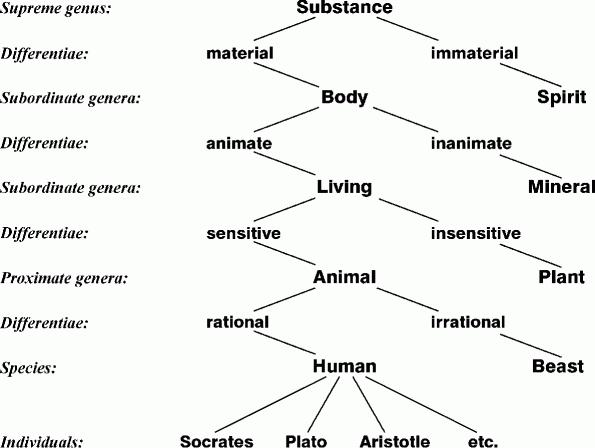
\includegraphics[scale=0.5]{./Images/tree.jpeg}

{\footnotesize \it Tree of Porphyry, taken from Cohen (2007)}
\end{center}

\noindent Many philosophical constructed languages that came before Atlan suggested or employed a so-called taxonomical ontology. Many of these are inspired by a diagram invented by the 3rd century Neoplatonist Porphyry when explaining Aristotle’s Categories (Porphyry, 300), called the Porphyrian tree (Franklin, 1986). In the Categories, Aristotle outlines a broad ontology of human apprehension, classifying everything that can be the subject or predicate of a statement into 10 categories: substance, quantity, quality, relation, place, time, position, state, action, affection (Aristoteles, 40). The Porphyrian tree (shown below) shows how a human falls into these categories, by showing different bifurcations from the first five categories (Cohen, 2007): 

Before Aristotle, similar ontological categorisations were made by the Vaiseshika school (Padārtha) (Stanford University, 2019) and the Stoic school, and after him numerous other thinkers, including Plotinus (430, 2019), Kant (Categories) (1781, 1998), Hegel  (1812, 1975), Peirce (1867), Husserl (1900, 1993) and Whitehead (categorial scheme) (1929, 2010). Not to mention folk ontologies, such as the Bantu nominal classes (Bleek, 1862–69) and the common distinction between animate and inanimate. All of these mostly were not taxonomical, however, and have been discussed extensively, but it is not the purpose of this paper to further investigate these discourses.  

There is, however, one specific notion within these categorisations which Atlan will incorporate, namely that of the {\it triadic categorisation} of Being. In Hegel, this comprises 1) Being (mind, consciousness, sensation), 2) Essence (Other, duality) and 3) Notion (synthesis, reference). In Peirce, these equate to Firstness (Quality, feeling, consciousness), Secondness (Reaction) and Thirdness (Meaning, representation). Atlan incorporates this through three degrees of removing from the speaking subject (see chapter 6.2). The first degree can be combined with the semantic prime for ‘person’ (´EJ´ \ej) to mean ‘I’ (´EJ.AM´ \ej \am), the second degree to mean ‘you’ (EJ.UN \ej \un) and the third to mean ‘he / she / they’ (´EJ.AJ´ \ej \aj), as well as other primes like place, time and demonstratives. 

A more explicit taxonomical ontology makes use of a so-called hierarchical classification. The idea of a ‘perfect’ or philosophical language was a popular idea during the enlightenment, being discussed by Bacon, Descartes, and Newton as a part of a widespread desire for a language that does not confuse the speaker’s understanding of reality or distort the natural order present in it (Eco, 1994, pp. 209-227).2 

The core idea of such a language is that it would build its words by adding different letters for every hierarchy of meaning. This way, related words would sound similar. There is, however, always a necessary degree of arbitrariness to such a system, since the arbitrary choice has to be made of what categories are specified by adding a limited set of different letters. These would have to be made from scratch, not based on previous languages, as to avoid confusion caused by natural language. These languages are known as a priori, and Atlan will be a priori as well, even though its contents are sourced from data from many natural languages but recombined in an attempt to circumvent natural language confusion.  

The first serious attempts at this ideal were made by George Dalgarno in his {\it Ars signorum} (1661, 1968) and John Wilkins in his \textit{Essay Towards a Real Character and a Philosophical Language} (1668, 1968). Initially, the two collaborated on a philosophical oligosynthetic language, but they couldn’t agree on whether to make the taxonomy encyclopaedic or build compound words from a small set of primes. Wilkins published his own version based on the former and Dalgarno the latter. Dalgarno’s language sadly never caught on, perhaps because the explanation of the linguistic working of the language was shrouded in philosophy which explained the structure \footnote{We hope this is not the case for this book as well.}. 

Wilkin’s language found a bit more recognition, being originally taken seriously by the Royal Society, with an attempt to finish the language after his death by a designated committee. It too, however, slowly lost interest in people and descended into oblivion  (FrathWiki, Ars Signorum, n.d.). Its taxonomical classification was structured to encompass every animal, plant, mineral and artifact. He achieved this by setting up an ingenious taxonomical tree to indicate the relations and bifurcations of meaning, along with a system of hierarchically adding vowels and consonants to specify differences and species within different categories. 

Wilkins regarded the language presented in his essay as just a draft, although he provides 2,030 different primitives, as well as a 15,000-word list for different English words but admits that it should be worked out by different teams of scientists to work out different concepts within their respective disciplines. His collaboration with the Royal Society was largely part of that attempt. Later on, Wilkin’s taxonomy went on to inspire Roget’s Thesaurus (1805) and later on Diderot and d’Alembert’s Encyclopaedia (1759).  

The idea was met with a lot of criticism as well. Voltaire criticised the optimism of the people attempting to create such a language in the form of the character Dr. Pangloss in his satire \textit{Candide} (1759, 1963). Jorge Luis Borges wrote an essay criticising taxonomical categorisations in general and Wilkin’s language specifically (1942) in which he mocks different instances of arbitrary classification by mentioning a fictional Chinese taxonomy called the \textit{Celestial Emporium of Benevolent Knowledge}. This list contains some very culture-specific, arbitrary and absurd categories such as ‘those belonging to the Emperor’, ‘those that have just broken the vase’ and ‘those that from afar look like flies’. This criticism seems like a bit of a stretch, because Wilkins put in a systematic effort to make a coherent classification, and this is not as arbitrary or absurd as Borges’ fictional classification. The linguist George Lakoff supports this claim by stating that many non-western cultures use classifications similar to European ones (Lakoff, 1987). Borges does point out that a successful execution of the idea could in theory have many benefits: ‘‘Mauthner points out that children would be able to learn this language without knowing it be artificial; afterwards, at school, they would discover it being an universal code and a secret encyclopaedia’’ (Blevins, n.d.). 

Foucault was inspired by Borges’ essay to write his book \textit{The Order of Things} (1966, 2010, p. preface) in which he analyses the social grounding of epistemic assumptions. He argues that implicit norms within intellectual communities determine thought and influence which topics are researched, and which are not, and how the established bias influences the interpretation of the data that is found. These assumptions and norms are bound to cultural and historic settings, and periodically go through reforms as a result of paradigm shifts. This is a strong blow to the aspiration of a universal classification of the universe. Borges claims that this is because: ‘‘we do not know what sort of thing the universe is’’. Metaphysicians and phenomenologists might differ on this, however, as will be discussed in chapter 3 of this essay.  

Besides this, Wilkins’ system has the disadvantage of only having a limited number of differences and species that can be specified because of the limited phonology. Atlan will be more similar to Dalgarno’s language, in that it will not drive its words through a hierarchical process of taxonomy, but rather by combining primes at will, allowing for exponentially more semantic combinations than are possible in Wilkin’s system. 

Another problem of Wilkin’s language is that words with similar meanings have very similar pronunciations, to the point of confusion. Modern information theory warns of this (Norman, n.d.), and Eco even identified that Wilkins himself made such a mistake, confusing {\it Gade} (barley) for {\it Gape} (tulip) (1994, p. 249). This would hinder the language’s intelligibility when mishearing can easily change important nuances in definition, as well as making is harder to speak fluently, because any speaker would have to work through tables and flowcharts in their minds while simultaneously talking, without making any mistakes. The language would also be very intolerant of subtle shifts in pronunciation and phrasing that tend to occur naturally within languages over time, because this would cause the whole encyclopaedic house of cards to come crashing down. 

Atlan will not have this problem, because its semantic primes are syllables instead of phonemes, and Atlan’s phonemic inventory is built to accommodate variation in phonetic approximation and sound shifts within its 14 archetype letters, without causing confusion or ambiguity. 

The philosopher Deleuze and psychoanalyst Guatarri proposed an alternative to arborescent (tree-like, hierarchical) epistemic networks like employed by Wilkins and Dalgarno, namely that of a {\it rhizome}, an analogy with a decentralised plant root network (1980, 2019). Such a model does account for bifurcations and conceptual relatedness but is more modal and allows for more complex interlinking than mere hierarchy. It would also fit the philosopher Quine’s idea of an interrelated epistemic ‘web of beliefs’ (Ney, 2014), as well as Wittgenstein’s claim that concepts are not clearly delineated, but rather surrounded by a ‘corona’ of associated concepts (1953, 2010, p. p. 181). 

Because of this, the main ontology seems to be better off using a combinatory system, which would allow for endless recombination and web-like relationships between similar words. This however doesn’t mean arborescent taxonomy should be completely abandoned. The most relevant modern case of taxonomical classification is that of natural species, although individual species don’t have clear demarcations and are loosely defined by their ability to produce fertile offspring (Nature Publishing Group, n.d.). Genetic diversification happened through bifurcation, known as {\it speciation}. The reverse, different species merging into one through hybridisation, called {\it despeciation}, does sometimes occur (including among early hominins), but is exceedingly rarer (Junior, 2018). Because of this, the evolutionary tree of life is primarily arborescent. 

Modern biological taxonomy employs the following hierarchical classification: life – domain – kingdom – phylum – class – order – family – genus – species (Biology Dictionary, 2017). Atlan’s biological lexicon is constructed along this framework, using semantic primes to describe different bifurcations, inspired by the Latin etymologies employed in binomial nomenclature (a hangover from Latin being the academic {\it lingua franca}). These binomial nomenclatures only mention the genus and species names of an organism, and words to designate species can re-occur in other genera to identify other species, adding to the parsimony of terms required to name all creatures within this system. 

Atlan shall have separate primes for the categories: \textit{virus, bacteria, archaea, plants, amoebas, fungi, animals.} In chapter 4 of this essay, a few culturally universal animal terms are identified, and these will be reduced to: \textit{mammal, fish, bird, worm, reptilian, insect.} Other animals could be reduced to their descriptions: sponges could be designated as foam-animals, starfishes to star-animals, snakes to legless-reptiles, amphibians to mucus-reptiles, molluscs to shell-animals, jellyfish to mucus-animals etc.  


Chemical molecules could be named by formalising a translation of the IUPAC nomenclature of organic chemistry from the originally Greek roots (IUPAC, 2021). Just like Wilkin’s language, Atlan will be dependent on scientists and specialists of different kinds of professions to add formalisations of their respective jargon nomenclatures to the lexicon in order to fully flesh out its lexicon. 

The reason why such a systematic description of reality claiming to be universal might be problematic, could be that it claims to have an objective image of reality, while all human thought, individual or collective, will always be fundamentally sourced from subjective experience. The philosopher Thomas Nagel described this by saying that there is no \textit{view from nowhere}\ (1989), while such a taxonomy appears to claim this anyway. The fact is that human concepts always have a necessary degree of arbitrariness because of the limited resolution of our conceptual boundaries. A taxonomical ontology implies the possibility of grasping some fundamental reductionist principle inherent to reality, while failing to see that many human concepts are emergent phenomena. The linguistic concept of an ‘organism’ cannot be reduced to a collection of organic molecules, because it is their complicated interplay that generates the multiple properties that pertain to an emergent system of self-preservation that humans call a single organism (Brigandt \& Love., 2017). On a microscopic level however, the clear boundaries of any single individual become fuzzy. It is because human life does not generally take place within a microscopic paradigm, that our concepts don’t have this level of detail. Reality is never described objectively, but always relative to the individual(s) observing and describing their reality. Humans appear to be ‘at the centre’ of their own language and understanding of reality. 

\section{The anthropocentricity of language}

Language and ontology are strongly entwined with one another: an ontological system is dependent on the words available to name its parts, and likewise a language is built from the set of concepts, relations, abstractions and ‘things’ that are captured by its lexicon  (Moltmann, 2017) (Boucon, 2019). Though by far not being the only elaboration on this idea, the Sapir-Whorf hypothesis is the most well-known inference that has been drawn from it. In short, this idea postulates that the range and limits of a person’s thought are determined by the language they speak. The strong version of this claim, linguistic relativism contends that all of human thought is fundamentally determined by language (linguistic determinism), resulting in some thoughts being lost and modified through translation or even untranslatable. It treats language as a fixed set of cognitive tools that acts as a constraint on the individual. This view, however, doesn’t enjoy a scholarly consensus (Whorf, 1956).  

However, this conception of language seems to be monolithic and extra personal instead of dynamic and dependant on individuals and their fluid interactions. It is challenged when presented with the fact that people within the same language can have vastly different ontologies, philosophies and vocabularies, depending on their individual personalities, interests and social environment, and the fact that individual people can learn multiple different languages and express their thoughts through them, nonetheless. Multilingualism is, however, noted to create within an individual, multiple linguistic ‘personæ’ for the different spoken languages, where one’s way of formulating thoughts and uttered sentences are altered by the individual characteristics of the different languages  (Pavlenko, 2006). 

Perhaps the influence that language has on the thoughts of its speaker can be likened to how putting on different glasses can alter one’s perception but does not change the fundamental scene being perceived through them. Sunglasses block out UV light, tinted glasses block out certain colours, different lenses shift the focus to what is near and other to what is far etc.: they all suppress some elements and amplify others, but they never change the basic composition of what is being perceived (if we discount virtual reality glasses). 

Using this metaphor, the purpose of Atlan is somewhat similar to being a clear, untainted, undeformed, unbiased pair of linguistic glasses, for as far as this is possible. Every single person’s eyes are different, and the glasses of their native language might be more or less similar to Atlan’s. The question then becomes: what constitutes this clear human experience that becomes tainted by language?  

First, we must realise that language itself is ontologically dependant on the total sum of living speakers. A dead, forgotten or undeciphered language cannot be said to currently exist in the same way that a living language like English exists. It might be revived in the future through the reconstruction of its linguistic information, but it only comes back into being when living humans are again able to read, write or speak the language. Furthermore, Wittgenstein’s private language argument states that a language is a fundamentally social thing, and that a purely personal language is therefore by definition impossible (1953, 2010, pp. \S 243-271). Language is a complicated system of communicating all kinds of mental information, like thoughts, feelings, intentions, physical data \&c., for all kinds of different purposes, like cooperation, social bonding, problem solving . In individual growing up in solitude or alongside animals never has the need nor possibility to learn and use a language, because there are no other humans around to converse with. After having passed the critical period of language acquisition without ever having learned a human language, an individual will never again be able to do so later in life (Robson, 2002).  

Therefore, language is an inherently human thing, that emerged from the transferring of information from one person’s individual experience to another’s. Phenomenal cues, like the sound of words, the rhythm of speech, facial expressions and gestures are used as an interpersonal bridge between the private mental worlds of the separate individuals. Someone can both hear themself talking, as well as someone else: language exists in a shared phenomenal space, whereas inner thought is private. Language then becomes a highly codified system of phenomenal metaphors. The sound of a specific word is not the same as the information it codifies, but is consistently associated with the referred phenomenon, in the form of an abstracted ‘concept’. 

Atlan should thus have an ontology that is built off the subjective human experience, when regarded in a social context and in direct contact with its physical environment. This immediately brings a degree of anthropocentricity with it, because words relating to the human psyche, body, daily life, social environment etc. will be given higher priority than the myriad of concepts and jargon within specialized disciplines that are less directly related to the everyday human experience. Moreover, humans should be able to think, talk and understand fluidly in a language, and not be required to consciously perform complicated linguistic computations within their heads while using the language. 

 

\section{Phenomenological ontology and qualia} 

Subjective experience is ultimately prior to any claim, idea, observation, connection \&c that can be communicated about reality. Anything in the world has to first present itself to us humans through phenomenal, subjective experience, before we can abstract it and understand it as an ‘objective’ phenomenon. However, the mainstream scientific metaphysical framework has, up to now, consistently been materialist, physicalist and reductionist. When it does acknowledge the existence of mind, it often does so in greatly unsatisfactory manner by employing some version of dualism, with the mind being metaphysically separate from the physical, but somehow miraculously still having epistemological and sensory access to it and the ability to manipulate it (moving one’s body at will) and be manipulated by it (physical alterations to the body or the ingestion of physical substances can alter the mental perception). When confronted with these problems, science will often try to explain the connection through a functionalist account of the neural network and a materialist explanation of the composition of our neurons, but always failing to close the explanatory gap to how this material process constitutes phenomenal experience. This is most painfully brought to light by the Hard Problem of Consciousness, the insurmountable chasm between a mechanistic description of neurology and the subjective experience of what it ‘feels’ like to exist as a conscious entity. Heidegger, building off the first phenomenological philosophy of Husserl, already warned of this in his own time halfway the 20th century, he called it \textit{Seinsvergessenheit}, the ‘forgottenness of Being’ (1962, 2019). Somehow the abstractions of reality that were derived from experience have gotten a higher ontological priority than the original experience itself, the ‘objective’ is regarded with a higher esteem than the ‘subjective’. It is beyond the purposes of this essay to explain why this happened and why it is metaphysically self-contradictory. Therefore, building off the premise of linguistic anthropocentricity established in the previous chapter, I shall relate the relevance of the subjective phenomenal experience to the construction of a universal human ontology in the current chapter. 

A famous thought experiment regarding the irreducibility of experience is called ‘Mary’s room’ (Jackson, 1982). It imagines a hypothetical scientist named Mary who (disregarding ethical concerns for the sake of the thought experiment) is raised in an exclusively black and white environment for her whole life, and educated about the science of colour perception, without ever seeing colour herself. She would have learned all there is to know about the physics of light, the biology of light receptors in the eye and the neural processing of visual information in the brain. The thought experiment then asks us: if Mary was to then leave her black and white environment and step outside and see colours for the first time in her life, would she learn anything new from experiencing, for example, the colour red for the first time? Could she have known its qualitative experience before she left the black and white room? Philosophers generally agree that she could not have known (the ‘knowledge argument’) (Nida-Rümelin \& Conaill, 2019). The same thought experiment could be extended to other subjective sensory perceptions like smell, taste, touch and sound and by extension even emotions and altered states of consciousness.3 Therefore, these ‘subjective’ qualitative aspects of experience appear to be fundamental and irreducible, modern philosophers call them ‘qualia’ (Tye, 2021). Since the coining of the term qualia in 1929 by C.I. Lewis, the concept has remained mostly confined to longwinded debate within the philosophy of mind.  

The formalisation of qualia is done by taking an ‘objective’ scale such as the spectrum of light frequencies, and then mapping phenomenal experience onto this by taking as a fundamental unit the smallest perceptible difference. Classically, qualitative experience is divided into the five physical senses: \textit{vision, hearing, smell, taste and touch.} In this essay I will supplement these with affective emotional experience and altered states of consciousness (the subjective experience of being stoned, drunk or tripping seems to be irreducible, they can be vaguely described when compared to sober consciousness, but to know the qualia of the experiment, one must take these substances personally). Because the language is oligosynthetic (see chapter 1 of the essay), the main purpose of this chapter is identifying the basic building blocks of the different types of qualia (vision, sound, taste, scent, physical sensation, emotion and consciousness states), which can then be combined into more nuanced qualitative descriptions.

\subsection{Vision}

\begin{center}
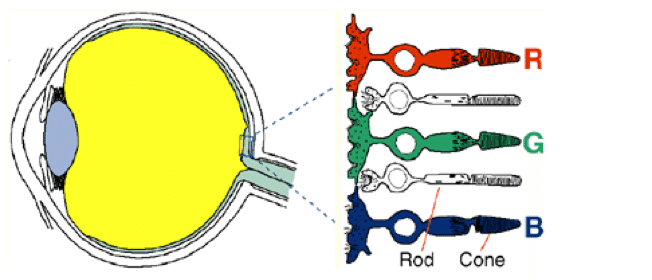
\includegraphics[scale=0.3]{./Images/eyes.jpeg}

{\it \footnotesize Cones of the human eye. From Mafalda (2017)}

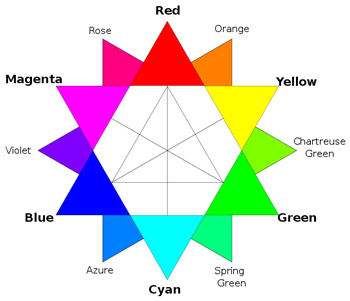
\includegraphics[scale=0.4]{./Images/colorwheel.jpg}

{\it \footnotesize Wheel of colour. From Judge (2012)}
\end{center}

\noindent Firstly, colour is the most straightforward, because it is already commonly divided into primary, secondary and tertiary colours. In psychophysical colorimetry the primary colours red, green and blue are regarded as being \textit{complete}, that is, constituting all human perceptible colours when combined along an axis of light to dark (additive light mixing), yet also being \textit{imaginary}, meaning only existing subjectively as qualia, while not being distinguishable as primaries through ‘objective’ measurement (Mac-Evoy, 2007). A standard human eye contain three types of light receptor cones, one for each of the three colours. 

All qualia that exist as polarities on a spectrum will be reduced to a semantic prime for the spectrum, combined with the particles for \textit{positive/high, neutral} and \textit{negative/low.} Translating this into an oligosynthetic semantic colour inventory, we would get the following (capitalised letters representing some as of yet undetermined but fixed assigned syllable): 

\vspace{0.1cm}

SHADES: 
\begin{itemize}

\item    Black/dark: JE.LAS \je \las (= negative + brightness) 

    \item White/light: FO.LAS \fo \las (= positive + brightness) 
\end{itemize}
\quad

PRIMARY: 
\begin{itemize}

    \item Red: EL \el 

    \item Green: OS \os 

\item Blue: UL \ul 
\end{itemize}
\quad


\noindent SECONDARY AND TERTIARY (RGB is chosen as fixed order): 

\begin{itemize}
\item   Orange: EL.OS \el \os 

\item   Cyan: OS.UL \os \ul 

\item   Magenta: UL.EL \ul \el 

\item   Orange: EL.OS.EL \el \os \el 

\item   Chartreuse green: EL.OS.OS \el \os \os 

\item   Spring green: OS.UL.OS \os \ul \os 

\item   Azure: OS.UL.UL \os \ul \ul 

\item   Violet: EL.UL.UL \ul \el \ul 

\item   Rose: EL.UL.EL \ul \el \el 
\end{itemize}

In 1969, anthropologist Brent Berlin and linguist Paul Kay published their book \textit{‘Basic Color Terms’} in which they proposed their research concerning the prevalence and development of different colour terms in languages from around the world (Berlin \& Kay, 1969). They proposed a chronological scheme of seven evolutionary stadia through which languages generally add colour terms to their lexicon. These are as follows: 

\begin{itemize}
\item Stage I: dark-cool (>‘black’) \& light-warm (>‘white’) 

\item Stage II: red 

\item Stage III:  green OR yellow 

\item Stage IV:  green AND yellow 

\item Stage V:  blue 

\item Stage VI:  brown 

\item Stage VII:  purple, pink, orange or gray 
\end{itemize}

Atlan, needing to conform to constraint 1, cultural neutrality, should thus contain these colours in its lexicon. Stage I-V have already been accounted for, and stage VI and VII can be covered by the combination of the colours from the earlier stages (following the order of shade-XYZ and primary-secondary-tertiary): 

\begin{itemize}
    \item Brown: red + green + blue  = ´EL.OS.UL´ \el \os \ul 

    \item Pink: white + red à = ´FO.LAS.EL´ \fo \las \el 

    \item Gray: colour + brightness + neutral = ´KAL.UJ.LAS´ \kal \uj \las 
\end{itemize}

All other colours and shades can be achieved using this combinatory system. One might argue that not all languages have the same lexical colour inventory, and some make more or less distinctions than English, but it should be noted that having a word for a specific colour is not the same as being able to perceive these different colours and their (subtle) differences (weak linguistic determinism, see chapter 1). Within the line of thought of linguistic determinism, one could argue that learning to speak Atlan, as having this colour system, would gift the speaker with an intuitive understanding of the composition of phenomenal color. 

Besides colour, three-dimensional shape is the other primary irreducible element within vision, constituting what in cognitive science is known as Gestalt (Rollinger \& Ierna, 2019). This term is also applicable to proportional ‘shapes’ or patterns within other qualia, like a musical melody. Visual shape can be geometrically reduced to lines/sides (1D), corners, surfaces (2D), angles and volumes (3D), making use of numerals to specify the quantities of these elements, as well as spatial prepositions to indicate relative location. This, however, will be further expounded upon in chapter 4 of the book, on Atlan’s numerals and mathematics.  


\subsection{Sound}

\noindent Sound is commonly divided into three elements:

\begin{itemize}
\item   The frequency of the soundwave, phenomenally corresponding with \textit{pitch}; 

\item   The amplitude of the soundwave, phenomenally corresponding with \textit{volume};

\item   The shape of the soundwave, phenomenally corresponding with \textit{timbre}.

\end{itemize}

\begin{center}
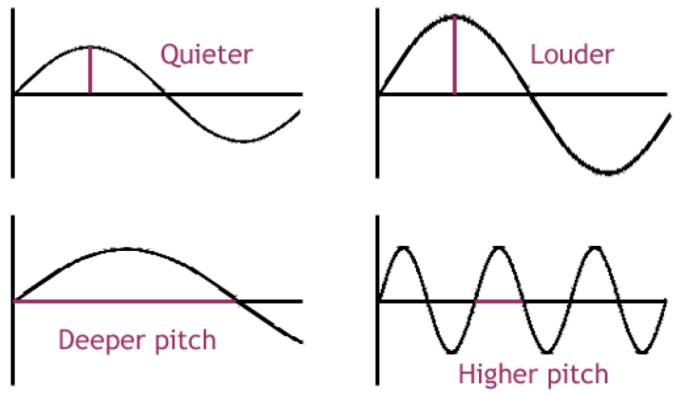
\includegraphics[scale=0.5]{./Images/Frequency.jpg}

{\it \footnotesize Frequency visualised. From Mata (2015).}
\end{center}


\begin{center}
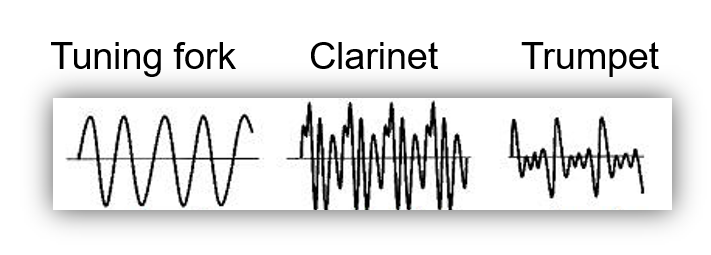
\includegraphics[scale=0.6]{./Images/Timbre.jpeg}

{\it \footnotesize Timbre. From SimplifyingTheory (n.d.).}
\end{center}


\begin{wrapfigure}[8]{r}{0.4\textwidth}
\includegraphics[scale=0.35]{./Images/pitch.jpg}

{\it \footnotesize Figure 3: The Chromatic Circle. From Wikimedia (2022).}

\end{wrapfigure}

\noindent Music theory almost universally divides pitch into a scale of notes, which repeats at the octave, where the ratio to the first note of the previous scale is 2:1. Western music uses the \textit{diatonic} scale, comprised of specifically alternating whole and half steps, and which is \textit{heptatonic} because it is comprised of 7 notes, before repeating at the octave (8th). There are a total of 12 half note steps within an octave, which comprise the \textit{chromatic} scale. Chromatic notes are specified relative to the \textit{natural} (\natural) heptatonic scale, by indicating a half step lower by a \textit{flat} (\flat) and a half step higher by a \textit{sharp}  (\sharp). 



The diatonic scale is not the most prevalent musical scale in the world, however, but rather the \textit{pentatonic} scale (five notes) (Encyclop\ae dia Britannica, inc., n.d.). However, a pentatonic scale fits neatly within a heptatonic scale, for example: C–D–E–G–A is a pentatonic scale which only omits the notes F and B. Because of this, Atlan shall use a system based on the Western heptatonic scale, while remaining culturally neutral because this system also accommodates the more common pentatonic scale. If it were to use the pentatonic scale as the standard, the heptatonic scale would be an extended modification, which would be quite clumsy seeing as Western music is so vast and globalised. 

Notes will be indicated with a context-dependent optional semantic prime for \textit{note/pitch} in front of the note name. The combination {\it note} + the first 7 numerals (see chapter 6.2) can be taken to represent the 7 notes (heptatonic: \textit{IP, OP, UP, IK, OK, UK, IM,} pentatonic: \textit{IP, OP, UP, OK, UK}). This will also make calculating musical intervals more intuitive because it will only require simple mental subtraction. 

Sharp will be indicated by \textit{pitch-positive} (also designating \textit{high} in the context of sound frequency) and flat (also indicating \textit{low} in the context of sound frequency) by \textit{pitch-negative.} Double sharps and double flats could be created by reduplicating \textit{positive/negative} respectively. Microtonal notes (which fall in between the chromatic notes) could be accounted for as follows: half-sharp -PN, half-flat -NP, three-quarter-sharp  -PNP, three-quarter-flat -NPN. Major and minor could be designated by the semantic primes for \textit{happy} and \textit{sad} (see the subchapter Emotions), and the seven scale modes could simply be numbered. Harmonic music theory is way too elaborate and complicated to cover fully in this paragraph, however it could be fairly easily constructed from the building blocks presented here. 

Volume is a lot simpler: within music theory it is known as dynamic, and divided into loud (Italian: \textit{forte, f}) and soft (Italian: \textit{piano, p}), further nuanced by the prefix medium (Italian: \textit{mezzo}), and by introducing a three-degree scale of intensity \textit{(ppp, pp, p, mp, mf, f, ff, fff)}. Adopting this system, Atlan can specify volume by combining the semantic prime for \textit{volume} with \textit{positive, medium, negative,} and a \textit{comparative/superlative} system, which will also be applied in other places of the language: \textit{X, more X, most X.} Changes in dynamic (growing louder, \textit{crescendo}, or softer, \textit{decrescendo}) can be described by the semantic primes for \textit{becoming} combined with \textit{more-volume-positive/ negative.} 

Finally, timbre, corresponding with the specific shape of the soundwave pattern, has an almost infinite range of possible combinations. This is why in language, terms that denote timbre are always metaphoric approximations, describing the sound with words that denote phenomena unrelated to sound when taken literally, but have a similar phenomenal quality to the sound (e.g., piercing, dark, bright), or are related to the origin of the sound (e.g., nasal, metallic). P. Sesuni analysed 45 studies on different timbre terms in English, Japanese, French, Czech, Swedish, Dutch, Finish, Spanish and German, and from these, identified 59 different descriptors (see appendix 1) (Susini, Carron, Rotureau, Dubois, \& Misdariis, 2017). 

Because these are all semantically reducible to non-sound-related terms, Atlan will not have any semantic primes specific to timbre, but rather use these and other timbre-descriptors, preceded by the semantic prime denoting \textit{sound}, combined with an adjective-marker. When occurring in a clearly sound-related context, the \textit{sound} prime may even be omitted, as there might not be any semantic confusion when it is already obvious that the adjective refers to a sound. 


\subsection{\it Taste and Scent}

\noindent Taste and scent are strongly correlated because both rely on chemoreceptors (molecule-detectors) (Reina, 2022) , with the main difference between the two that taste is perceived by the tongue and concerns solid and liquid matter, while smell goes through the nose and pertains to gaseous matter. Because many tastes have an olfactory counterpart, tastes may be marked by adding the semantic prime \textit{taste} and scents with \textit{smell.} 

The five main taste categories are \textit{sweet, sour, bitter, salt, umami}  (Deutsch, 2019), which will be separate semantic primes in Atlan. These may double as scents when marked with \textit{smell} instead of \textit{taste}. The true range of scents and tastes, just like timbre, is overwhelmingly complex, thanks to the many different possible molecules and combinations between these. Thus, further nuances in flavour and aroma may be constituted in similar fashion to timbre, referring either to the source of the smell or taste (e.g., floral, alcoholic, vanilla-like), or a comparable quality (e.g., harsh, sharp, mellow). Spice is not a taste, but rather a form of phenomenal pain, because it is registered by chemical nociceptors (molecule-pain receptors). Spice can thus be constituted by combining the semantic prime for \textit{pain} with \textit{taste/smell.} Of course, different taste or scent designators can be combined at will to create even more nuanced descriptions. 

\subsection{Physical sensation}

The physical senses cover a broad range of different sensations in different parts of the body (Reina, 2022). All terms for physical sensation shall be preceded by the semantic prime for \textit{feeling.} This prime might also be used psychologically/affectively in other contexts. Mechanoreceptors sense physical deformation like pressure, touch, stretch and motion but also sound, corresponding to vibrations of the ear drum. Because sound has already been covered, it will not be counted among physical sensation. Combined with the range \textit{positive-neutral-negative,} these will yield the following terms:  

\begin{itemize}
\item   \textit{Contact}: pressure – touch – barely touch  

\item   \textit{Tension}: stretched – relaxed – contracted  

\item   \textit{Texture}: rough – normal – smooth 
\end{itemize}

More detailed textural descriptions can be made by combining with different material primes mentioned in the conclusion of this essay. Terms for motion of touch will be mentioned in chapter 5.4.  

Thermoreceptors report \textit{temperature} and nociceptors pain, as stated earlier regarding the taste of spice. \textit{Pleasure} does not have a specific receptor but is rather constituted by neurotransmitters fired in the brain in reaction to certain perceptions, however, is often seen as the opposite polarity of pain (Kringelbach \& Berridge, 2009). These will thus we constituted as follows:  


\begin{itemize}
\item   \textit{Temperature}: hot –tepid – cold  

\item   \textit{Valence}: pleasure – neutral – pain  

\item   \textit{Wetness}: wet – moist/damp – dry 
\end{itemize}

Somatic sense refers to the outside of the body, and visceral sense to internal organs. These will be codified by the semantic primes for \textit{outside} and \textit{inside} respectively.   

\begin{itemize}
	\item Internal \textit{tension}: bloating/swollen – normal pressure – cramp  
\end{itemize}

Proprioceptors sense the relative position of body parts, and the vestibular system registers the orientation of the entire body in space, perceived as \textit{balance} (Proske \& Gandevia, 2012).  

\begin{itemize}
	\item \textit{Balance}: grounded – balanced – out of balance.  

	\item Dizziness: \textit{balance-negative + turning.} 

	\item Motion sickness:  \textit{ balance-negative + motion } 

	\item Seasickness \textit{balance-negative + sea.} 
\end{itemize}


\subsection{Emotions}

\begin{center}
	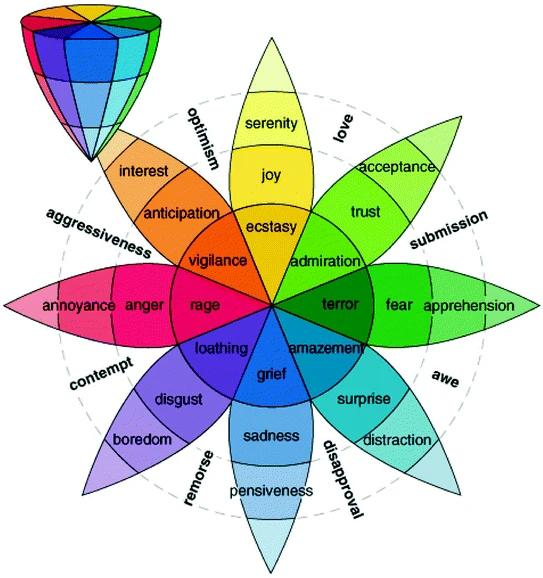
\includegraphics[scale=0.45]{./Images/emotions.jpg}

	{\it \footnotesize Plutchik's wheel of emotions. From Gkonou et al. (2015)}
\end{center}

\noindent In 1980, the American psychology professor Robert Plutchik published a geometric model of the different basic emotions  (Plutchik, 1980). Each pair of geometrically opposing sections constitute emotional antipoles. The justification for his classification is psychoevolutionary and traces the origins of the different affects to behavioural responses that would emerge naturally in reaction to different challenges and attractors encountered by humans and other animals (see appendix 2) (Plutchik \& Kellerman, Theories of emotion, 1980).  

Again, using the grid of positive – neutral – negative, the eight basic emotions and their respective three degrees of intensity can be covered: 

\begin{enumerate}
\item   Anger 

\item   Anticipation 

\item   Joy 

\item   Trust 

\item   Fear 

\item   Surprise 
	
\item   Sadness 

\item   Disgust
\end{enumerate}

Intermediary emotions can be achieved by combining with other emotions or semantic primes (see appendix 3). 

\subsection{Consciousness states}

The different consciousness states of the human psyche are the hardest qualia to pin down. The NOBA Project, an online Psychology teaching platform, identifies the following (Teener \& Teeny, n.d.): 

\begin{enumerate}
\item   Consciousness 

\item   Awareness 

\item   Hypnosis 

\item   Dissociation 

\item   Trance / depersonalisation 

\item   Sleep 

\item   Hallucination 

\item   Depression 

\item   Stimulation / excitation
\end{enumerate}
 

\noindent To complete the pallet of consciousness, I shall add the following: 
\setcounter{enumi}{9}
\begin{enumerate}
\item   Reason / abstract logos / logic 

\item   Memory 

\item   Desire / will 

\item   Conscience (moral) 

\item   Intuition / instinct 

\item   Imagination / creativity 

\item   Understanding
\end{enumerate}

\noindent These can be combined with various other semantic primes to constitute various psychological terms (see appendix 4).  

To sum up this chapter, to cover most all human qualia, Atlan will employ a set of qualia-specific atoms combined with some more general semantic atoms (see appendix 5).

\section{Universal Semantics}

Now that the basic constituents of human psychic experience have been accounted for, the different concepts within mankind’s material understanding of the world have been largely neglected. This is what this chapter aims to rectify. In needing to satisfy Atlan’s first constraint (human universality / cultural-linguistic neutrality), the semantic inventory would need to contain semantic primes or syntheses of these that cover a set of concepts shared cross-linguistically.  

The comparative linguist Morris Swadesh published his commonly used list of 207 lexicostatistically universal concepts in 1952 (see appendix 6) (Swadesh, 1952), after making a series of revised versions. It is used to compare relatedness between languages by analysing the quantitative overlap in their words for the different Swadesh terms. Atlan builds on this list as a guideline, grouping related concepts, reducing some and adding other terms where possible (see chapter 6 of the book). 

Another, more abstracted summary of the basic semantic elements of human language is given by the Natural Semantic Metalanguage developed by the cross-cultural linguist Anna Wierzbicka (Goddard \& Wierzbicka, Meaning and Universal Grammar: Theory and Empirical Findings., 2002). Though different languages might express concepts in different ways, the semantic content of NSM is divided into 65 semantic primitives, spread over 16 categories (see appendix 7) (Levisen \& Waters, 2017). 

Atlan uses this classification as a guideline, and the semantic primitives will be synthesised with the Swadesh list. Within NSM, semantic ‘molecules’ are terms that can be reduced to the 65 primitives, or ‘atoms’, but are often used to build more complicated meanings. Where the atoms are abstract, the molecule are more concrete. There is, therefore, an added value of listing such molecules to minimise complexity, because molecule-composite words would be a lot more longwinded when all their semantic atoms had to be stated individually. The research into this topic is still underdeveloped, but a few sets of supposedly universal semantic molecules have been proposed. The website of the university of Griffith mentions the following universal semantic molecules (see appendix 8) (Griffith University, n.d.).  

This lexicon already bears a striking similarity to the Swadesh list. Cliff Goddard identifies a few additional semantic molecules in English (Goddard, 2012). These will be incorporated because of the globalised distribution of Anglo-American culture and language. In a video-essay he adds several other mostly culture-bound molecules (NSMLab, 2021). Atlan will synthesise these lists into the semantic inventory (see appendix 9).  

 

\section{Concluding remarks}

In this chapter, I have introduced the problem of an oligosynthetic ontology to constitute Atlan’s semantics in a way that respects the constraints of cultural neutrality, unambiguity and form from function. I discussed previous attempts at a system like this and other systems of classification, and the critical discourse around these. I discussed the role of the human perspective within human language, and the relationship between language ontology and subjective thought. I dove into the philosophical movement of phenomenology and argued for the irreducibility of qualitative experience (qualia). I went on to map out the state-space of qualitative experience, and mapped out how different qualia could be reduced into an oligosynthetic combinatory system of word-generation. I then referenced different academic projects that mapped out a minimal account of cross-culturally universal irreducible concepts, which will be added to the language in order to respect the constraint of cultural neutrality and the premise of linguistic anthropocentricity. Chapter 6.2 of the book contains the final semantic inventory of Atlan’s 490 semantic syllable-primes, sorted into conceptually related semantic categories. These are sorted into having maximally similar initial letters and modelled by AI to be as similar as possible to various different natural languages, weighed by their linguistic genealogy and total amount of speakers, making the lexicon semi-a priori sourced. 


\section{Appendix}
\noindent 1. Timbre descriptions in natural languages.

\begin{center}
	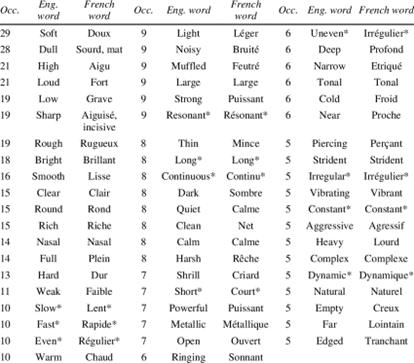
\includegraphics[scale=0.6]{./Images/timbre.jpg}
\end{center}



\noindent 2: Psycho-evolutionary classification of animal emotions 

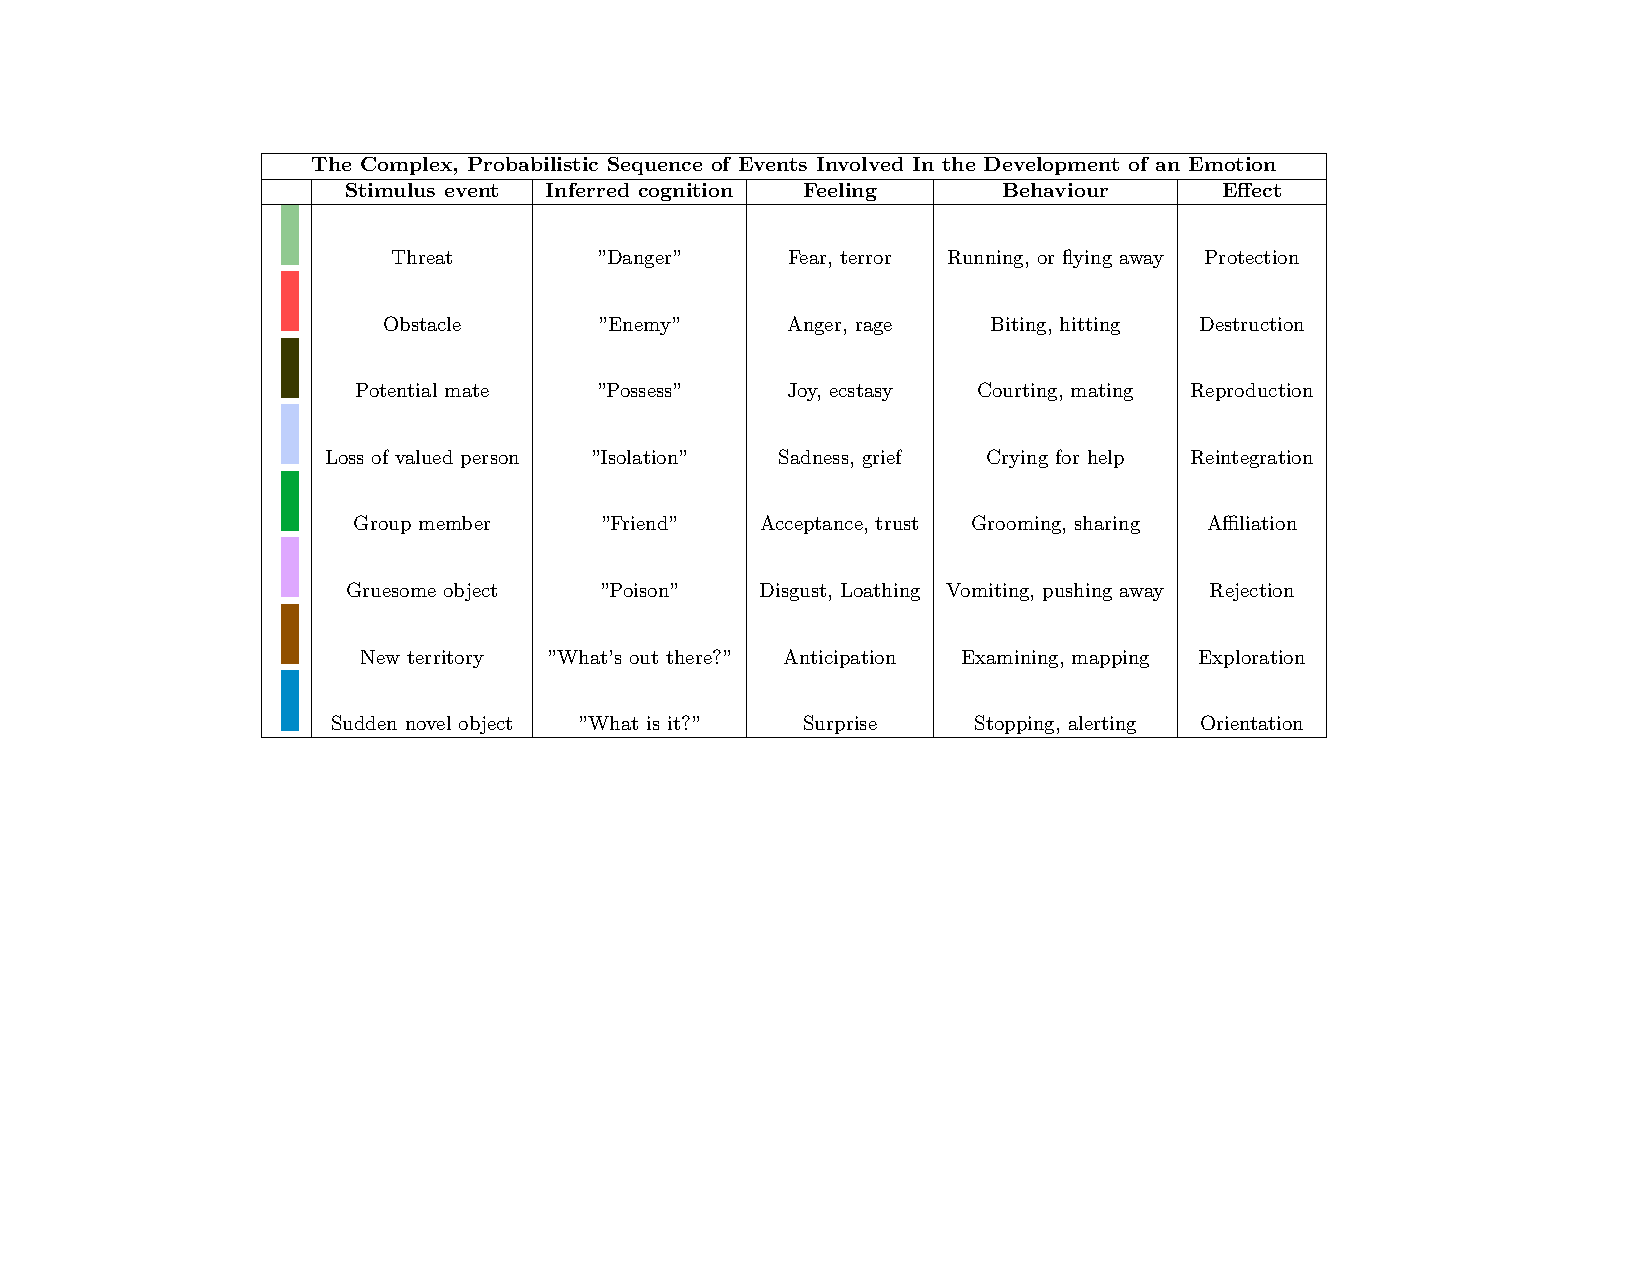
\includepdf[scale=1.4,pagecommand={}, width = 0.8\pagewidth, angle= 90]{./Mainmatter/tabelfeelings.pdf}

%\resizebox{1\textwidth}{!}{
%\begingroup

%\begin{tabular}{|l|c|c|c|c|c|}
%\hline

%\multicolumn{6}{|c|}{ \bf  The Complex, Probabilistic Sequence of Events Involved In the Development of an Emotion} \\ 

%\hline

%& {\bf Stimulus event} 
%	

%& {\bf Inferred cognition} 
%	

%& {\bf Feeling} 
%	

%& {\bf Behaviour} 
%	

%& {\bf Effect} \\
%\hline
% 
%\definecolor{softgreen}{RGB}{144,201,144}
%{\color{softgreen} \rule{0.3cm}{1cm}}
%	

% & Threat 
%	

%& "Danger" 
%	

%& Fear, terror 
%	

% & Running, or flying away 
%	

%& Protection \\ 

% 
%\definecolor{softred}{RGB}{255,74,74}
%{\color{softred} \rule{0.3cm}{1cm}}
%	

%& Obstacle 
%	

%& "Enemy" 
%	

%& Anger, rage 
%	

%& Biting, hitting 
%	

% & Destruction\\ 

% 
%	
%\definecolor{softbrown}{RGB}{57,57,0}
%{\color{softbrown} \rule{0.3cm}{1cm}}


%& Potential mate 
%	

%& "Possess" 
%	

%& Joy, ecstasy 
%	

%& Courting, mating 
%	

%& Reproduction\\ 

% 
%	
%\definecolor{softblue}{RGB}{191,207,252}
%{\color{softblue} \rule{0.3cm}{1cm}}

%& Loss of valued person 
%	

%& "Isolation" 
%	

%& Sadness, grief 
%	

%& Crying for help 
%	

%& Reintegration\\ 

% 
%	
%\definecolor{brightgreen}{RGB}{0,166,55}
%{\color{brightgreen} \rule{0.3cm}{1cm}}

%& Group member 
%	

%& "Friend" 
%	

%& Acceptance, trust 
%	

%& Grooming, sharing 
%	

%& Affiliation\\ 

% 
%	
%\definecolor{softpurple}{RGB}{222,168,255}
%{\color{softpurple} \rule{0.3cm}{1cm}}

%& Gruesome object 
%	

%& "Poison" 
%	

%& Disgust, Loathing 
%	

%& Vomiting, pushing away 
%	

%& Rejection\\ 

% 
%\definecolor{brawn}{RGB}{145,80,0}
%{\color{brawn} \rule{0.3cm}{1cm}}
%	

%& New territory 
%	

%& "What's out there?" 
%	

%& Anticipation 
%	

%& Examining, mapping 
%	

%& Exploration\\ 

% 
%\definecolor{blu}{RGB}{0,138,200}
%{\color{blu} \rule{0.3cm}{1cm}}
%	

%& Sudden novel object 
%	

%& "What is it?" 
%	

%& Surprise 
%	

%& Stopping, alerting 
%	

%& Orientation\\ 

%\hline
%\end{tabular}
%\endgroup
%}


\noindent 3.Combinatorics of Atlan’s emotional and semantic atoms 

\begin{itemize}
\item   Optimism = anticipation + joy 

\item   Love = joy + trust 

\item   Shame embarrassment = fear + disgust 

\item   Thoughtfulness = serene + interest 

\item   Thankfulness = serene + acceptance 

\item   Pride = admire + self 

\item   Faith / belief = trust + know 

\item   Extravagance = ecstasy + distracted 

\item   Daringness = trust + anticipation 

\item   Rejection / refusal = not + accepting 

\item   (In)security = (not +) trust + self  

\item   Discouraged = passive + not + trust + anticipation 

\item   Bewildered = surprise + apprehension 

\item   Critical / sceptical = not + trust + know  

\item   Frustration = anger + distraction  

\item   Jealousy = desire + annoyed 

\end{itemize}


\begin{multicols}{2}
\noindent 4. Combinatorics of Atlan’s consciousness and semantic atoms  
\begin{itemize}
\item   Unconscious = not + consciousness 

\item   Sub-conscious = below + consciousness 

\item   Ego = feeling + self 

\item   Self-consciousness = consciousness + self 

\item   Narcissism = admiration + self 

\item   Selfishness / egotism = interest + self 

\item   Depersonalisation = feeling + not + self 

\item   Ego-death = feeling + self + death 

\item   Derealisation = feeling + not + contact + reality  

\item   Libido = desire + sex 

\item   Arousal = stimulation + sex 

\item   Orgasm = ecstasy + sex 

\item   Deep sleep = sleep + not + consciousness 

\item   Dreaming = sleep + consciousness 

\item   Lucid dreaming = dreaming + consciousness + awareness 

\item   Enlightenment = consciousness + light / bright 

\item   Bliss = ecstasy + peace 

\item   Mystical experience = consciousness + God 

\item   Sensory overload = feel + excitation + positive 

\item   Peace = excitation + neutral 

\item   Numbness = feel + excitation + negative 

\item   Euphoria = feeling + good 

\item   Dysphoria = feeling + bad 

\item   High = feeling + cannabis + excitation + positive 

\item   Stoned = feeling + cannabis + excitation + negative 

\item   Tipsy = feeling + alcohol + neutral 

\item   Drunk = feeling + alcohol + positive 

\item   Understand = reason + grasp 

\item   Aha-Erlebnis = feeling + understanding 

\item   Empathy = feeling + other 

\item   Social awareness = awareness + social 

\item   Intelligent = reason + positive 

\item   Dumb = reason + negative 

\item   Guilt = conscience + bad 

\item   Know-how = understanding + action 

\item   Wisdom = understanding + life 
\end{itemize}
\end{multicols}

\noindent{5. Overview of qualia-related atoms}
\begin{multicols}{2}

\begin{itemize}
\item   Negative 

\item   Neutral  

\item   Positive  

\item   Colour 

\item   Brightness 

\item   Red 

\item   Yellow 

\item   Blue 

\item   Sound 

\item   Volume 

\item   Become, transform 

\item   Note/pitch 

\item   7 note-names corresponding with the numbers 1-7 

\item   (…) 

\item   More (comparative)  

\item   Most (superlative) 

\item   Smell 

\item   Taste 

\item   Sweet 

\item   Sour 

\item   Bitter 

\item   Salty 

\item   Umami 

\item   Feeling / affect 

\item   Contact 

\item   Tension 

\item   Texture 

\item   Temperature 

\item   Valence 

\item   Wetness 

\item   Outside 

\item   Inside 

\item   Balance 

\item   Turn 

\item   Move 

\item   Sea 

\item   Anger 

\item   Anticipation 

\item   Joy 

\item   Trust 

\item   Fear 

\item   Surprise 

\item   Sadness 

\item   Disgust 

\item   Consciousness 

\item   Awareness 

\item   Hypnosis 

\item   Dissociation 

\item   Trance/depersonalisation 

\item   Sleep 

\item   Hallucination 

\item   Depression 

\item   Stimulation / excitation 

\item   Reason / abstract logos  

\item   Memory 

\item   Desire 

\item   Conscience (moral) 

\item   Intuition / instinct 

\item   Below 

\item   Self 

\item   Death 

\item   Reality 

\item   Sex 

\item   Not 

\item   Light 

\item   God 

\item   Value judgement  

\item   Grasp 

\item   Social  
\end{itemize}
\end{multicols}

\noindent  6. Swadesh 207 list of universal human concepts 

\begin{multicols}{2}
\begin{enumerate}
\item   I 

\item   you (singular) 

\item   they (singular) 

\item   we 

\item   you (plural) 

\item   they (plural) 

\item   this 

\item   that 

\item   here 

\item   there 

\item   who 

\item   what 

\item   where 

\item   when 

\item   how 

\item   not 

\item   all 

\item   many 

\item   some 

\item   few 

\item   other 

\item   one 

\item   two 

\item   three 

\item   four 

\item   five 

\item   big 

\item   long 

\item   wide 

\item   thick 

\item   heavy 

\item   small 

\item   short 

\item   narrow 

\item   thin 

\item   woman 

\item   man (adult male) 

\item   man (human being) 

\item   child 

\item   wife 

\item   husband 

\item   mother 

\item   father 

\item   animal 

\item   fish 

\item   bird 

\item   dog 

\item   louse 

\item   snake 

\item   worm 

\item   tree 

\item   forest 

\item   stick 

\item   fruit 

\item   seed 

\item   leaf 

\item   root 

\item   bark (of a tree) 

\item   flower 

\item   grass 

\item   rope 

\item   skin 

\item   meat 

\item   blood 

\item   bone 

\item   fat (noun) 

\item   egg 

\item   horn 

\item   tail 

\item   feather 

\item   hair 

\item   head 

\item   ear 

\item   eye 

\item   nose 

\item   mouth 

\item   tooth 

\item   tongue (organ) 

\item   fingernail 

\item   foot 

\item   leg 

\item   knee 

\item   hand 

\item   wing 

\item   belly 

\item   guts 

\item   neck 

\item   back 

\item   breast 

\item   heart 

\item   liver 

\item   to drink 

\item   to eat 

\item   to bite 

\item   to suck 

\item   to spit 

\item   to vomit 

\item   to blow 

\item   to breathe 

\item   to laugh 

\item   to see 

\item   to hear 

\item   to know 

\item   to think 

\item   to smell 

\item   to fear 

\item   to sleep 

\item   to live 

\item   to die 

\item   to kill 

\item   to fight 

\item   to hunt 

\item   to hit 

\item   to cut 

\item   to split 

\item   to stab 

\item   to scratch 

\item   to dig 

\item   to swim 

\item   to fly 

\item   to walk 

\item   to come 

\item   to lie (as in a bed) 

\item   to sit 

\item   to stand 

\item   to turn (intransitive) 

\item   to fall 

\item   to give 

\item   to hold 

\item   to squeeze 

\item   to rub 

\item   to wash 

\item   to wipe 

\item   to pull 

\item   to push 

\item   to throw 

\item   to tie 

\item   to sew 

\item   to count 

\item   to say 

\item   to sing 

\item   to play 

\item   to float 

\item   to flow 

\item   to freeze 

\item   to swell 

\item   sun 

\item   moon 

\item   star 

\item   water 

\item   rain 

\item   river 

\item   lake 

\item   sea 

\item   salt 

\item   stone 

\item   sand 

\item   dust 

\item   earth 

\item   cloud 

\item   fog 

\item   sky 

\item   wind 

\item   snow 

\item   ice 

\item   smoke 

\item   fire 

\item   ash 

\item   to burn 

\item   road 

\item   mountain 

\item   red 

\item   green 

\item   yellow 

\item   white 

\item   black 

\item   night 

\item   day 

\item   year 

\item   warm 

\item   cold 

\item   full 

\item   new 

\item   old 

\item   good 

\item   bad 

\item   rotten 

\item   dirty 

\item   straight 

\item   round 

\item   sharp (as a knife) 

\item   dull (as a knife) 

\item   smooth 

\item   wet 

\item   dry 

\item   correct 

\item   near 

\item   far 

\item   right 

\item   left 

\item   at 

\item   in 

\item   with 

\item   and 

\item   if 

\item   because 

\item   name 
\end{enumerate}
\end{multicols}




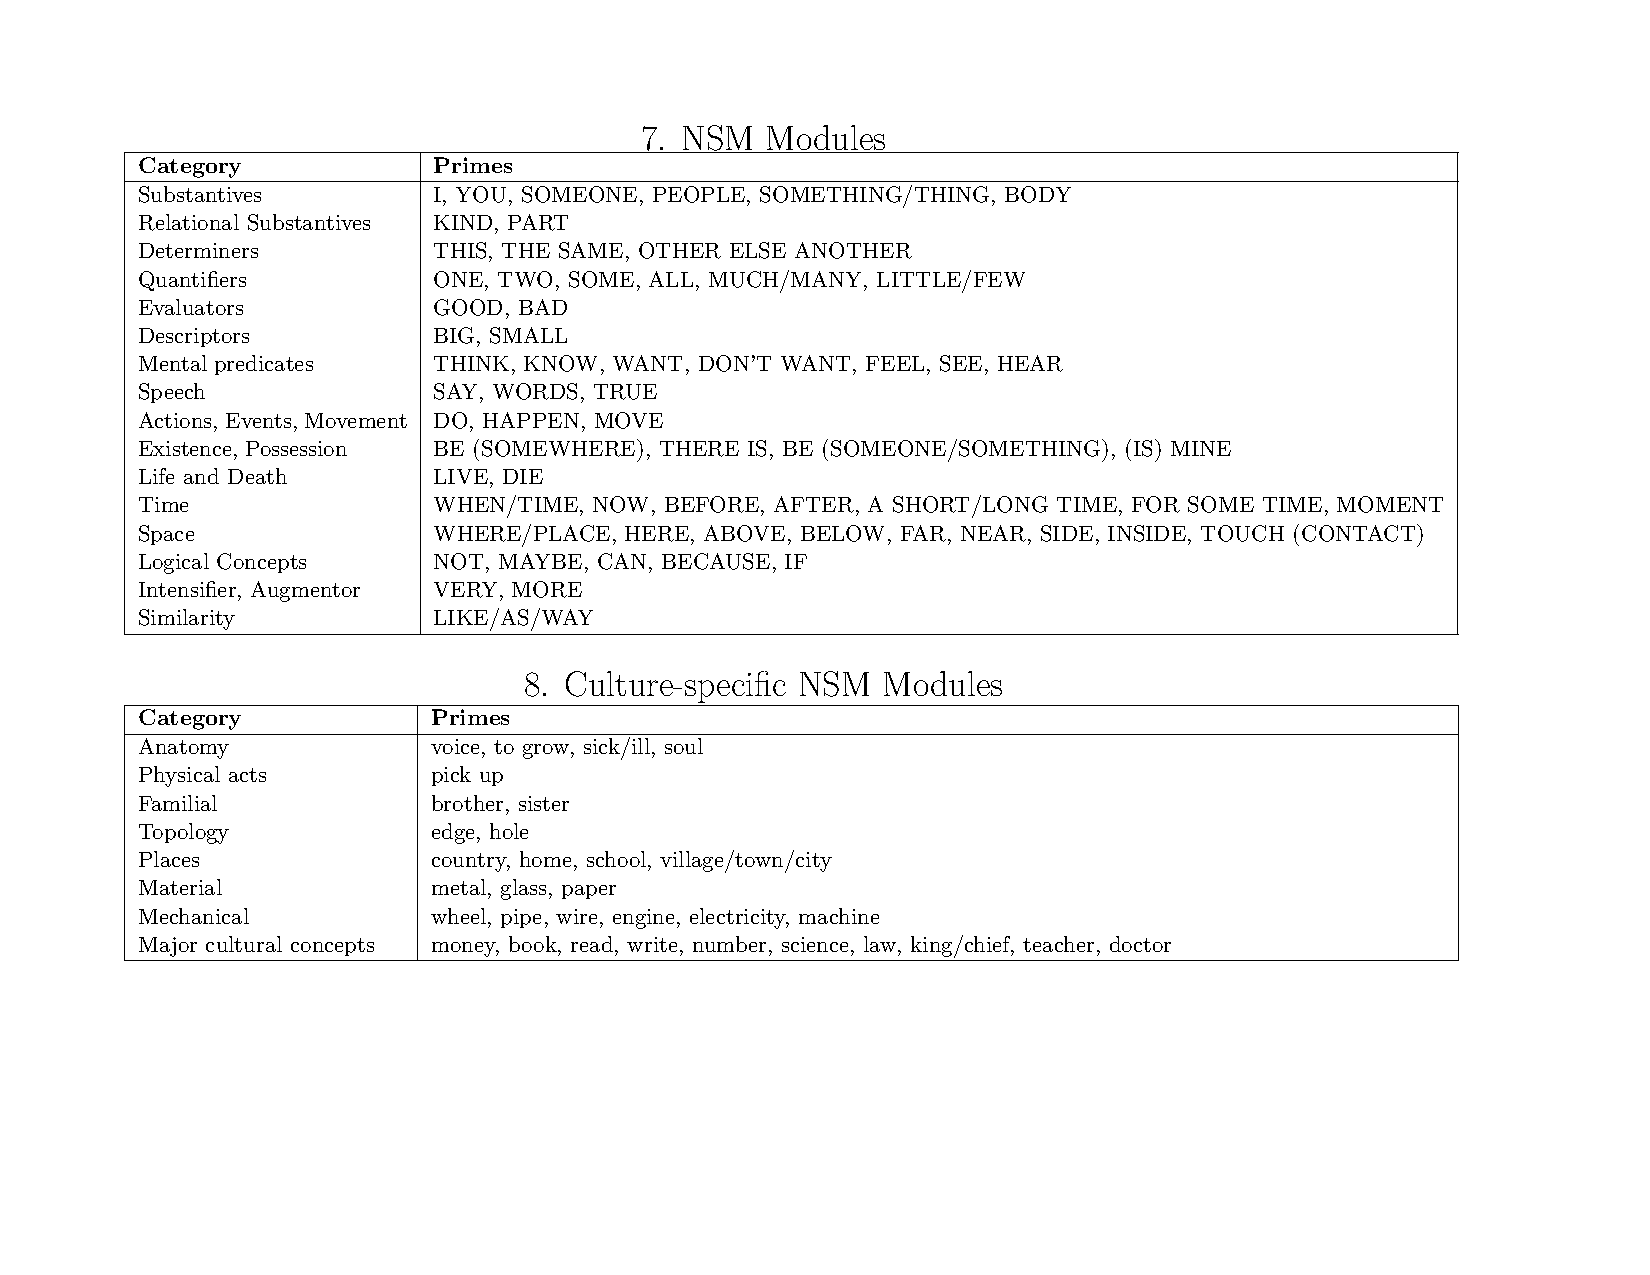
\includepdf[scale=1.4,pagecommand={}, width = 0.8\pagewidth, angle= 90,pages=1]{./Mainmatter/nsmatoms.pdf}

\pagebreak

\includepdf[scale=1.4,pagecommand={}, width = 0.8\pagewidth, angle= 90, pages=2]{./Mainmatter/nsmatoms.pdf}


%\resizebox{1\textwidth}{!}{
%\begin{tabular}{|c|c|}
%	\hline
%\textbf{Category}& 
%\textbf{Primes}\\ 
%\hline
%
%Substantives & 
%	
%
%I, YOU, SOMEONE, PEOPLE, SOMETHING/THING, BODY\\ 
%
%Relational Substantives & 
%	
%
%KIND, PART\\ 
%
%Determiners & 
%	
%
%THIS, THE SAME, OTHER~ELSE~ANOTHER\\ 
%
%Quantifiers & 
%	
%
%ONE, TWO, SOME, ALL, MUCH/MANY, LITTLE/FEW\\ 
%
%Evaluators & 
%	
%
%GOOD, BAD\\ 
%
%Descriptors&  
%	
%
%BIG, SMALL\\ 
%
%Mental predicates& 
%	
%
%THINK, KNOW, WANT, DON'T WANT, FEEL, SEE, HEAR\\ 
%
%Speech& 
%	
%
%SAY, WORDS, TRUE\\ 
%
%Actions, Events, Movement& 
%	
%
%DO, HAPPEN, MOVE\\ 
%
%Existence, Possession& 
%	
%
%BE (SOMEWHERE), THERE IS, BE (SOMEONE/SOMETHING), (IS) MINE\\ 
%
%Life and Death& 
%	
%
%LIVE, DIE \\
%
%Time& 
%	
%
%WHEN/TIME, NOW, BEFORE, AFTER, A SHORT/LONG TIME,FOR SOME TIME, MOMENT\\ 
%
%Space& 
%	
%
%WHERE/PLACE, HERE, ABOVE, BELOW, FAR, NEAR, SIDE, INSIDE, TOUCH (CONTACT)\\ 
%
%Logical Concepts& 
%	
%
%NOT, MAYBE, CAN, BECAUSE, IF\\ 
%
%Intensifier, Augmentor& 
%	
%
%VERY, MORE\\ 
%
%Similarity& 
%	
%
%LIKE/AS/WAY\\ 
%\hline
%
%\end{tabular}
%}
%
%\noindent 8. Proposed universal NSM modules
%
%\resizebox{1\textwidth}{!}{
%\begin{tabular}{|c|c|}
%\hline
%\textbf{Category}& 
%\textbf{Primes}\\ 
%\hline
%Body parts& 
%	
%
%hands, mouth, eyes, head, ears, nose, face, teeth, fingers, breast, skin, bones, blood\\ 
%
%Physical& 
%	
%
%long, round, flat, thin, hard, soft, sharp, smooth, heavy \\ 
%
%Spatial / physical& 
%	
%
%be on something, at the top, at the bottom, in the middle, in front of, around \\ 
%
%Environmental& 
%	
%
%sky, the Earth, sun, moon, stars, ground, during the day, at night\\ 
%
%Times& 
%	
%
%day\\ 
%
%Fire and water& 
%	
%
%water, fire\\ 
%
%Biological& 
%	
%
%creature, grow, egg, tail, wings, feathers \\ 
%
%Biosocial 
%& 
%	
%
%children, men, women, be born, mother, father, wife, husband\\ 
%
%Materials& 
%	
%
%wood, stone\\ 
%
%"Knowing" and "naming"& 
%	
%
%know (someone), be called\\ 
%
%"Doing"& 
%	
%
%hold, make, kill, breathe, sleep, sit, lie, stand, play, laugh, sing\\ 
%
%\hline
%\end{tabular}
%}
%
%\noindent 9. Culture-specific NSM modules
%
%\resizebox{1\textwidth}{!}{
%\begin{tabular}{|c|c|}
%\hline
%\textbf{Category}& 
%\textbf{Primes}\\ 
%\hline
%Anatomy& 
%	
%
%voice, to grow, sick/ill, soul\\ 
%
%Physical acts& 
%	
%
%pick up\\ 
%
%Familial& 
%	
%
%brother, sister\\ 
%
%Topology& 
%	
%
%edge, hole\\ 
%
%Places& 
%	
%
%country, home, school, village/town/city\\ 
%
%Material& 
%	
%
%metal, glass, paper\\ 
%
%Mechanical& 
%	
%
%wheel, pipe, wire, engine, electricity, machine\\ 
%
%Major cultural concepts& 
%	
%
%money, book, read, write, number, science, law, king/chief, teacher, doctor\\ 
%
%\hline
%\end{tabular}
%}
